\documentclass[10pt, a4paper]{article}

\usepackage{amsmath}
\usepackage{amssymb}
\usepackage{graphicx}
\usepackage{listings}
\usepackage{color}
\usepackage[section]{placeins}
\usepackage{paralist}

\definecolor{mygreen}{rgb}{0,0.6,0}
\definecolor{mygray}{rgb}{0.5,0.5,0.5}
\definecolor{mymauve}{rgb}{0.58,0,0.82}

\lstset{ %
  backgroundcolor=\color{white},
  basicstyle=\footnotesize,
  breakatwhitespace=false,
  breaklines=true,
  captionpos=b,
  commentstyle=\color{mygreen},
  escapeinside={\%*}{*)},
  extendedchars=true,
  keepspaces=true,
  keywordstyle=\color{blue},
  rulecolor=\color{black},
  showspaces=false,
  showstringspaces=false,
  showtabs=false,
  stepnumber=2,
  stringstyle=\color{mymauve},
  tabsize=2,
}

\hyphenation{GENITOR}

\newcommand*{\titleGM}{\begingroup
\hbox{ 
\hspace*{0.2\textwidth} 
\rule{1pt}{\textheight} 
\hspace*{0.05\textwidth} 
\parbox[b]{0.75\textwidth}{ 

{\noindent\Huge\bfseries Solving Travelling Salesman Problems using Genetic
 Algorithms}\\[2\baselineskip] % Title
{\large \textit{SEM6120 - Assignment 2}}\\[4\baselineskip] % Tagline or further description
{\Large \textsc{Alexander D Brown (adb9)}} % Author name

\vspace{0.5\textheight} 
}}
\endgroup}


\title{Genetic Algorithms}
\author{Alexander D Brown (adb9)}

\begin{document}
\titleGM 
\tableofcontents
\newpage

\section{Introduction}
This report investigates the use of Genetic Algorithms to solve the Travelling
Salesman Problem, introducing both topics as well as previous research and 
techniques.

Following this the design for the solution implemented will be detailed,
focusing from high level system design to annotated code section to explain the
choice behind the implementation.

This implementation is then used to produced the results in
section~\ref{sec:results} which give an insight into the affects of different
crossover and mutation schemes on the performance of the genetic algorithm,
specifically looking at %TODO actually get some results to finish this.

Finally the author will draw conclusions from these results and %TODO I don't
% know what I'm going to do at this point.


\subsection{Genetic Algorithms}
Genetic algorithms are a biologically-inspired approach to heuristic search 
that mimic natural selection. Unlike many other evolutionary strategies and
evolutionary programming, they are not designed to solve a specific problem,
but are designed to solve the problem of optimisation which is made difficult
by substantial complexity and uncertainty\cite{Holland1992Adaptation}.

\subsection{Travelling Salesman Problem}
%TODO this section need citations.
The Travelling Salesman Problem is a well-known NP-hard optimisation problem
which asks the question: \textit{``Given a number of cities and the distances 
between these cities, find the shortest touch which visits each city exactly 
once and returns to the first city.''}

Assuming each city is connected to every other city, this problem reaches a
complexity of $O(n!)$ and is very resource intensive to brute force a problem
with any decent number of nodes quickly become too larger problem to solve
within a reasonable amount of time.

There are many heuristic algorithms which have been applied successfully to the
Travelling Salesman Problem, including both Evolutionary and Genetic 
Algorithms.

Though the nature of Genetic Algorithms are suited to the optimisation of a
Travelling Salesman Problem, normal methods of crossover and mutation cannot,
generally, be applied directly to the problem. The representation of 
chromosomes has to be ordered (i.e.\ each city must appear once and only once)
and additional methods of crossover and mutation have had to be designed for
these ordered chromosomes.

\newpage
\section{Design}
% TODO Introduction

\subsection{System Design}
% TODO
% Overall idea: modularise system
As with most coding problems with multiple options, a modular approach is
necessary to keep code quality high. This is typically done by defining
high-level interfaces for the changeable elements. In this case the obvious
three interfaces are:

%  - Define high-level classes for selection, crossover & mutation
\begin{enumerate}
\item Selection Scheme
\item Crossover Scheme
\item Mutation Scheme
\end{enumerate}

From these high-level classes, concrete sub-classes can be written to perform
the actual logic. An example of this would be a specific class for Order-1
based crossover.

%  - Use factories to generate specific classes based of input
This leaves the problem of how to accesses these classes based on an input
string; the easiest method for this is to use factories to access these 
classes, cutting down the number of specific imports required and centralising
the logic for creating them.

%  - Discuss the structure of graphs and ways to cut down the amount of memory
%    used.


\subsubsection{Language Choice}
Python was the choice of language, it is a dynamically typed language which 
provides several programming paradigms to work with, including procedural,
object-orientated and functional paradigms.

It is a language the author is very familiar with and has the advantage of
having many open source libraries to perform different scientific functions;
some of these libraries have been used in the course of this project, including
the popular \texttt{numpy} library for number processing and 
\texttt{matplotlib} to produce graphs.

The strange choice of \texttt{pygame} was made for the choice of displaying the
GUI, but this games library gives simple yet powerful access to OpenGL and also
manages platform dependencies.

\subsubsection{UML Class Diagram}

Figure~\ref{fig:uml} shows the initial UML Class diagram for this project.
There are some elements which break from typical object-orientated design,
noticeably the representation of nodes in a graph as a map of integers to a
turple of float, these parts are done so to re-use internal data structures of
the Python programming language to speed up the implementation of many 
features.

\begin{figure}[h]
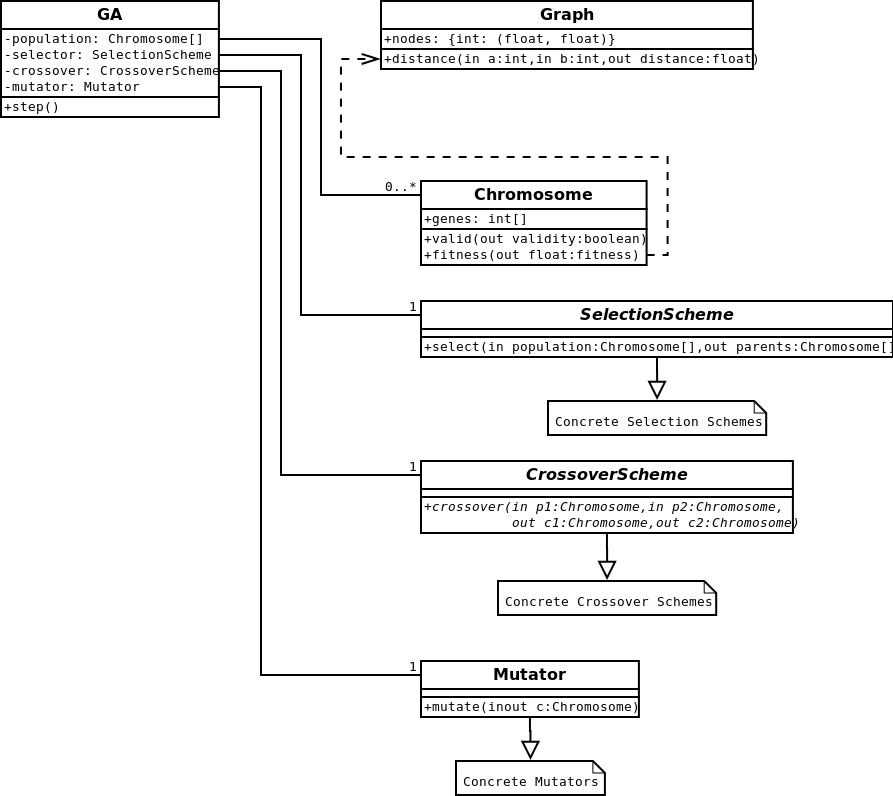
\includegraphics[width=\textwidth]{img/uml.png}
\caption{UML Class Diagram for the Genetic Algorithm}
\label{fig:uml}
\end{figure}

This design is such that factories exist to create selection schemes, crossover
schemes and mutators based on an input string to facilitate the switching of
these elements via command line arguments.

This design was slowly improved through the project; the
\texttt{CrossoverScheme} class implemented the \texttt{crossover} method, 
which then called a separate method, \texttt{do\_crossover}, to generate 
\texttt{c1} based on \texttt{do\_crossover(p1, p2)} and \texttt{c2} on 
\texttt{do\_crossover(p2, p1)} to make the processing more uniform. Subclasses
were still able to override the \texttt{crossover} method, but were encouraged
to implement a \texttt{do\_crossover} method unless the scheme required a
different behaviour of child generation.


\subsubsection{Representation of Graphs}

The actual of representation of a graph is a map of the node identifier to the
$x$ and $y$ co-ordinates of that node (as a tuple). This allows easy look up 
of nodes within the map to get the position of the node. This was chosen 
because of the representation of the problem in chromosomes - each gene 
represents a node in the graph.

With this representation, the fitness function would be the distance of the 
tour represented by these nodes:

\begin{equation}
d_{tour} = \sum^{N}_{i=0}{
  \begin{cases}
    d(n_i, n_{i+1}) & \text{if } i+n < N \\ 
    d(n_i, n_0)     & \text{else}
  \end{cases}
}
\end{equation}

Programatically, with the advantage of the functional and in-built elements of 
Python, this can be simplified to:

\lstset{language=Python}
\begin{lstlisting}[language=Python, caption=Distance of a tour]
def d_tour():
  # Move the first element of the array to the end.
  shifted = nodes[1:] + nodes[:1]
  return sum([distance(i, j) for (i, j) in zip(nodes, shifted)])
\end{lstlisting}

\subsection{Use of Functional Programming Paradigms}

As Python implements several different programming paradigms a lot of problems
can be solved with a different approach than other languages can. Both genetic
algorithms and the travelling salesman problem lend themselves towards a more
functional approach with a lot of list processing. Using Pythons list
comprehensions and the in-built list functions shortened the amount of code 
required and makes the code a lot easier to understand for those who are used 
to this approach.

A very good example of this is the method for evaluating chromosomes in a
population, returning a list sorted from the best to the worst:

\begin{lstlisting}[language=Python, 
                   caption=Using function elements to improve sustinctness and
                           readability]
def eval(population):
  return sorted(population, 
                key = lambda chromosome: chromosome.fitness())
\end{lstlisting}


\subsection{Crossover Strategies}

Three main types of crossover strategies were implemented for this research:

\begin{enumerate}
\item Cycle Crossover,
\item Order Crossover Operator,
\item M-Crossover Operator.%TODO\cite
\end{enumerate}

All three are designed to work with ordered chromosomes, meaning they can be
applied directly to the Travelling Salesman Problem without any modification.
%TODO for comparison a non-ordered strategy was implemented and modified.

\subsubsection{Cycle Crossover}

Cycle crossover is one of the simplest order-based crossover operators. Unlike
many other forms of order-based operators it make no effort to preserve parts 
of the parent chromosomes.

To produce a child, $c$, from parents $p_1$ and $p_2$ a randomly selected point
$i$ is chosen. The gene at $i$ in $p_1$ ($r = p_1(i)$) is removed and replaced 
with $p_1(i) = p_2(i)$. The position of the removed allele $r$ is found in 
$p_2$ such that $i = index(r, p_2)$. This process is repeated until a cycle
occurs (i.e. the removed allele $r$ is the same as the initially removed 
allele).

Figure~\ref{fig:cycle-crossover} shows this process step by step on two ordered
chromosomes. Note that it only by chance that parts of the tour are preserved.

\begin{figure}[h]
\centering
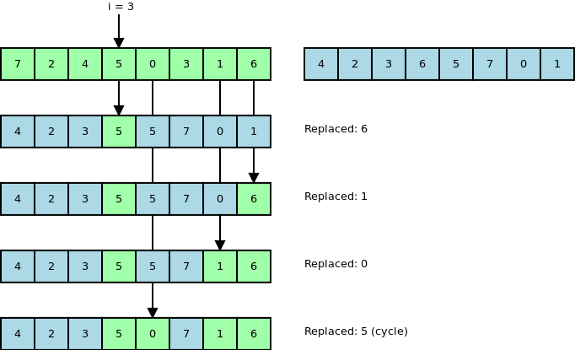
\includegraphics[width=0.8\textwidth]{img/cycle-crossover.png}
\caption{Cycle Crossover}
\label{fig:cycle-crossover}
\end{figure}


\subsubsection{Order Crossover Operator}

The order crossover operator is another simple order-based crossover operator.
Unlike cycle crossover, it preserves at least part of a tour from one of the
parents.

To produce a child, $c$, from parents $p_1, p_2$, a random segment from $p_1$ 
is appended to the remaining genes from $p_2$, omitting any alleles that are
also in the segment from $p_1$.

Figure~\ref{fig:order-crossover-operator} shows this process step by step on
two ordered chromosomes. Note that at least a part of the tour is always
preserved and that it is often the case that a part of a tour from $p_1$ and
$p_2$ is preserved in $c$.

\begin{figure}[h]
\centering
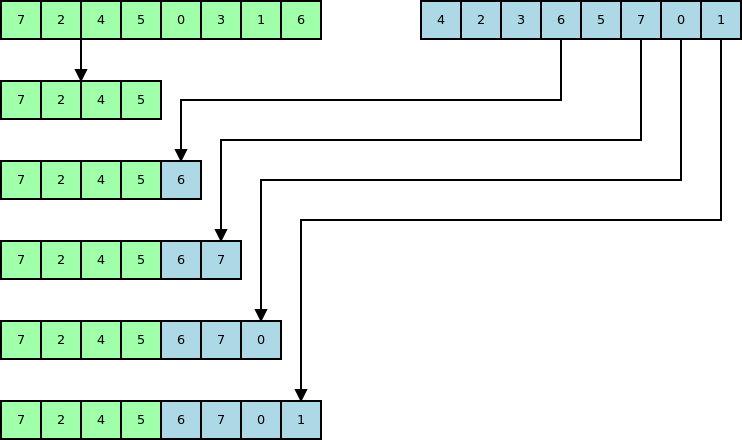
\includegraphics[width=0.8\textwidth]{img/order-crossover-operator}
\caption{Order Crossover Operator}
\label{fig:order-crossover-operator}
\end{figure}


\subsubsection{M-Crossover Operator}

The m-crossover operator\cite{Mudaliar2013Unraveling} produces multiple 
offspring ($C$) from parents $p_1, p_2$ then selects the best two from this 
process.

Like with the order crossover operator, this is based on segmenting the
chromosomes. However, both chromosomes are split into several segments. Every
segment of $p_1$ is inserted at any point in front, behind or between the
segments of $p_2$ and vice versa. The new, elongated chromosome is then
processed such that any allele in the added segment is removed from all other
segments to produce the child at that point.

The fitness of these children is then evaulated and the best two are carried 
forward as the offspring of these parents.

\begin{figure}[h]
\centering
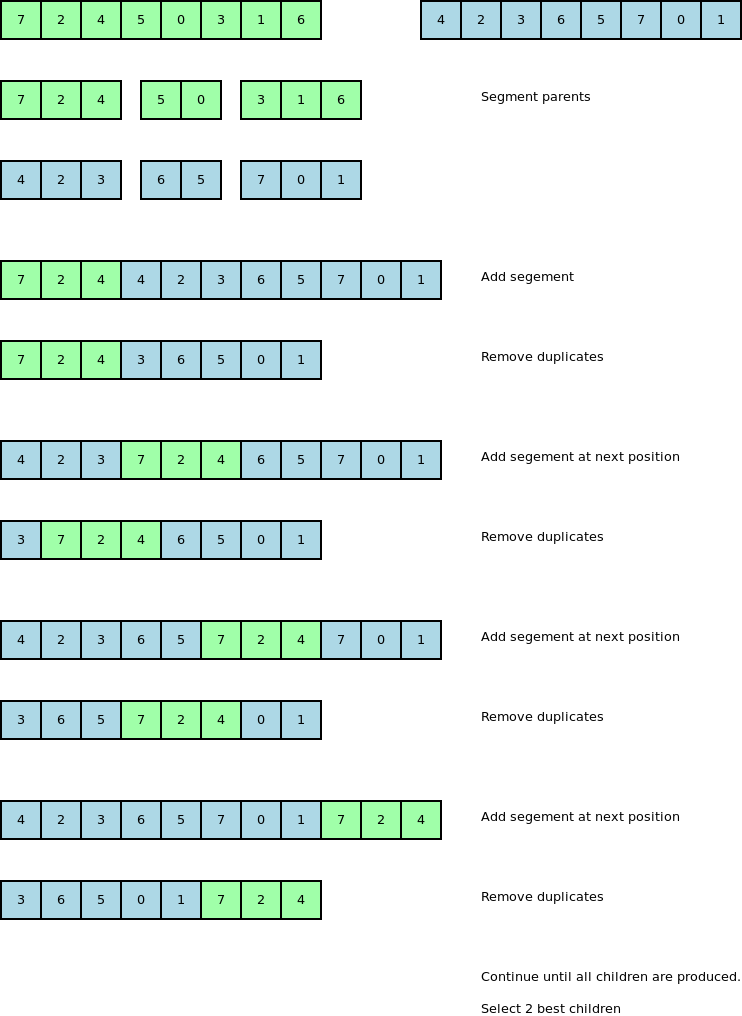
\includegraphics[width=0.8\textwidth]{img/m-crossover-operator}
\caption{M-Crossover Operator}
\label{fig:m-crossover-operator}
\end{figure}

 
\section{Results}
\label{sec:results}

\subsection{Best and Mean Population Fitness against Number of Generations}
%TODO

\subsection{Best and Mean Population Fitness against Runtime}
%TODO

\subsection{Convergence}
%TODO

\section{Conclusions}
%TODO


\bibliographystyle{plain}
\bibliography{citations}

\end{document}
